%  LaTeX support: latex@mdpi.com
%  For support, please attach all files needed for compiling as well as the log file, and specify your operating system, LaTeX version, and LaTeX editor.

%=================================================================
% pandoc conditionals added to preserve backwards compatibility with previous versions of rticles

\documentclass[,,,moreauthors,pdftex]{Definitions/mdpi}


%% Some pieces required from the pandoc template
\setlist[itemize]{leftmargin=*,labelsep=5.8mm}
\setlist[enumerate]{leftmargin=*,labelsep=4.9mm}


%--------------------
% Class Options:
%--------------------
%----------
% journal
%----------
% Choose between the following MDPI journals:
% acoustics, actuators, addictions, admsci, adolescents, aerobiology, aerospace, agriculture, agriengineering, agrochemicals, agronomy, ai, air, algorithms, allergies, alloys, analytica, analytics, anatomia, animals, antibiotics, antibodies, antioxidants, applbiosci, appliedchem, appliedmath, applmech, applmicrobiol, applnano, applsci, aquacj, architecture, arm, arthropoda, arts, asc, asi, astronomy, atmosphere, atoms, audiolres, automation, axioms, bacteria, batteries, bdcc, behavsci, beverages, biochem, bioengineering, biologics, biology, biomass, biomechanics, biomed, biomedicines, biomedinformatics, biomimetics, biomolecules, biophysica, biosensors, biotech, birds, bloods, blsf, brainsci, breath, buildings, businesses, cancers, carbon, cardiogenetics, catalysts, cells, ceramics, challenges, chemengineering, chemistry, chemosensors, chemproc, children, chips, cimb, civileng, cleantechnol, climate, clinpract, clockssleep, cmd, coasts, coatings, colloids, colorants, commodities, compounds, computation, computers, condensedmatter, conservation, constrmater, cosmetics, covid, crops, cryptography, crystals, csmf, ctn, curroncol, cyber, dairy, data, ddc, dentistry, dermato, dermatopathology, designs, devices, diabetology, diagnostics, dietetics, digital, disabilities, diseases, diversity, dna, drones, dynamics, earth, ebj, ecologies, econometrics, economies, education, ejihpe, electricity, electrochem, electronicmat, electronics, encyclopedia, endocrines, energies, eng, engproc, entomology, entropy, environments, environsciproc, epidemiologia, epigenomes, est, fermentation, fibers, fintech, fire, fishes, fluids, foods, forecasting, forensicsci, forests, foundations, fractalfract, fuels, future, futureinternet, futurepharmacol, futurephys, futuretransp, galaxies, games, gases, gastroent, gastrointestdisord, gels, genealogy, genes, geographies, geohazards, geomatics, geosciences, geotechnics, geriatrics, grasses, gucdd, hazardousmatters, healthcare, hearts, hemato, hematolrep, heritage, higheredu, highthroughput, histories, horticulturae, hospitals, humanities, humans, hydrobiology, hydrogen, hydrology, hygiene, idr, ijerph, ijfs, ijgi, ijms, ijns, ijpb, ijtm, ijtpp, ime, immuno, informatics, information, infrastructures, inorganics, insects, instruments, inventions, iot, j, jal, jcdd, jcm, jcp, jcs, jcto, jdb, jeta, jfb, jfmk, jimaging, jintelligence, jlpea, jmmp, jmp, jmse, jne, jnt, jof, joitmc, jor, journalmedia, jox, jpm, jrfm, jsan, jtaer, jvd, jzbg, kidneydial, kinasesphosphatases, knowledge, land, languages, laws, life, liquids, literature, livers, logics, logistics, lubricants, lymphatics, machines, macromol, magnetism, magnetochemistry, make, marinedrugs, materials, materproc, mathematics, mca, measurements, medicina, medicines, medsci, membranes, merits, metabolites, metals, meteorology, methane, metrology, micro, microarrays, microbiolres, micromachines, microorganisms, microplastics, minerals, mining, modelling, molbank, molecules, mps, msf, mti, muscles, nanoenergyadv, nanomanufacturing,\gdef\@continuouspages{yes}} nanomaterials, ncrna, ndt, network, neuroglia, neurolint, neurosci, nitrogen, notspecified, %%nri, nursrep, nutraceuticals, nutrients, obesities, oceans, ohbm, onco, %oncopathology, optics, oral, organics, organoids, osteology, oxygen, parasites, parasitologia, particles, pathogens, pathophysiology, pediatrrep, pharmaceuticals, pharmaceutics, pharmacoepidemiology,\gdef\@ISSN{2813-0618}\gdef\@continuous pharmacy, philosophies, photochem, photonics, phycology, physchem, physics, physiologia, plants, plasma, platforms, pollutants, polymers, polysaccharides, poultry, powders, preprints, proceedings, processes, prosthesis, proteomes, psf, psych, psychiatryint, psychoactives, publications, quantumrep, quaternary, qubs, radiation, reactions, receptors, recycling, regeneration, religions, remotesensing, reports, reprodmed, resources, rheumato, risks, robotics, ruminants, safety, sci, scipharm, sclerosis, seeds, sensors, separations, sexes, signals, sinusitis, skins, smartcities, sna, societies, socsci, software, soilsystems, solar, solids, spectroscj, sports, standards, stats, std, stresses, surfaces, surgeries, suschem, sustainability, symmetry, synbio, systems, targets, taxonomy, technologies, telecom, test, textiles, thalassrep, thermo, tomography, tourismhosp, toxics, toxins, transplantology, transportation, traumacare, traumas, tropicalmed, universe, urbansci, uro, vaccines, vehicles, venereology, vetsci, vibration, virtualworlds, viruses, vision, waste, water, wem, wevj, wind, women, world, youth, zoonoticdis 
% For posting an early version of this manuscript as a preprint, you may use "preprints" as the journal. Changing "submit" to "accept" before posting will remove line numbers.

%---------
% article
%---------
% The default type of manuscript is "article", but can be replaced by: 
% abstract, addendum, article, book, bookreview, briefreport, casereport, comment, commentary, communication, conferenceproceedings, correction, conferencereport, entry, expressionofconcern, extendedabstract, datadescriptor, editorial, essay, erratum, hypothesis, interestingimage, obituary, opinion, projectreport, reply, retraction, review, perspective, protocol, shortnote, studyprotocol, systematicreview, supfile, technicalnote, viewpoint, guidelines, registeredreport, tutorial
% supfile = supplementary materials

%----------
% submit
%----------
% The class option "submit" will be changed to "accept" by the Editorial Office when the paper is accepted. This will only make changes to the frontpage (e.g., the logo of the journal will get visible), the headings, and the copyright information. Also, line numbering will be removed. Journal info and pagination for accepted papers will also be assigned by the Editorial Office.

%------------------
% moreauthors
%------------------
% If there is only one author the class option oneauthor should be used. Otherwise use the class option moreauthors.

%---------
% pdftex
%---------
% The option pdftex is for use with pdfLaTeX. Remove "pdftex" for (1) compiling with LaTeX & dvi2pdf (if eps figures are used) or for (2) compiling with XeLaTeX.

%=================================================================
% MDPI internal commands - do not modify
\firstpage{1} 
\makeatletter 
\setcounter{page}{\@firstpage} 
\makeatother
\pubvolume{1}
\issuenum{1}
\articlenumber{0}
\pubyear{2024}
\copyrightyear{2024}
%\externaleditor{Academic Editor: Firstname Lastname}
\datereceived{ } 
\daterevised{ } % Comment out if no revised date
\dateaccepted{ } 
\datepublished{ } 
%\datecorrected{} % For corrected papers: "Corrected: XXX" date in the original paper.
%\dateretracted{} % For corrected papers: "Retracted: XXX" date in the original paper.
\hreflink{https://doi.org/} % If needed use \linebreak
%\doinum{}
%\pdfoutput=1 % Uncommented for upload to arXiv.org
%\CorrStatement{yes}  % For updates


%=================================================================
% Add packages and commands here. The following packages are loaded in our class file: fontenc, inputenc, calc, indentfirst, fancyhdr, graphicx, epstopdf, lastpage, ifthen, float, amsmath, amssymb, lineno, setspace, enumitem, mathpazo, booktabs, titlesec, etoolbox, tabto, xcolor, colortbl, soul, multirow, microtype, tikz, totcount, changepage, attrib, upgreek, array, tabularx, pbox, ragged2e, tocloft, marginnote, marginfix, enotez, amsthm, natbib, hyperref, cleveref, scrextend, url, geometry, newfloat, caption, draftwatermark, seqsplit
% cleveref: load \crefname definitions after \begin{document}

%=================================================================
% Please use the following mathematics environments: Theorem, Lemma, Corollary, Proposition, Characterization, Property, Problem, Example, ExamplesandDefinitions, Hypothesis, Remark, Definition, Notation, Assumption
%% For proofs, please use the proof environment (the amsthm package is loaded by the MDPI class).

%=================================================================
% Full title of the paper (Capitalized)
\Title{Proyecto Análisis Exploratorio de Datos: Calidad del Aire
(2004-2025)}

% MDPI internal command: Title for citation in the left column
\TitleCitation{Proyecto Análisis Exploratorio de Datos: Calidad del Aire
(2004-2025)}

% Author Orchid ID: enter ID or remove command
%\newcommand{\orcidauthorA}{0000-0000-0000-000X} % Add \orcidA{} behind the author's name
%\newcommand{\orcidauthorB}{0000-0000-0000-000X} % Add \orcidB{} behind the author's name


% Authors, for the paper (add full first names)
\Author{Adriana Marí López$^{}$, An Xueyao$^{}$, Cristhian Torrico
Castellon$^{}$}


%\longauthorlist{yes}


% MDPI internal command: Authors, for metadata in PDF
\AuthorNames{Adriana Marí López, An Xueyao, Cristhian Torrico Castellon}

% MDPI internal command: Authors, for citation in the left column

% Affiliations / Addresses (Add [1] after \address if there is only one affiliation.)
\address{%
$^{}$ \quad ; \\
}

% Contact information of the corresponding author
\corres{Correspondence: }

% Current address and/or shared authorship








% The commands \thirdnote{} till \eighthnote{} are available for further notes

% Simple summary

%\conference{} % An extended version of a conference paper

% Abstract (Do not insert blank lines, i.e. \\)
\abstract{La calidad del aire es un determinante clave de la salud
pública en entornos urbanos. El objetivo principal de este proyecto es
realizar un Análisis Exploratorio de Datos (AED) para comprender sus
patrones en Valencia, utilizando datos de 2004 a 2025. El trabajo aborda
la compleja tarea de consolidar, limpiar y estandarizar conjuntos de
datos heterogéneos provenientes de múltiples fuentes (Ayuntamiento de
Valencia y GVA). Se detalla un proceso de ingeniería de datos, aplicando
técnicas de imputación de series temporales para gestionar robustamente
los valores ausentes. El punto central del análisis es la derivación del
Índice de Calidad del Aire (ICA) Europeo para la última década. Sobre
esta variable clave, se aplican técnicas de análisis descriptivo
univariante y bivariante para examinar la distribución del ICA.
Asimismo, se exploran sus patrones espaciales, temporales y de
comportamiento, concluyendo con un análisis de correlación para estudiar
la relación entre el ICA y diversos factores explicativos, tanto
meteorológicos como humanos.}


% Keywords
\keyword{Calidad del Aire; Análisis Exploratorio de Datos (AED); Índice
de Calidad del Aire (ICA); Valencia; Preprocesamiento de Datos; Limpieza
de Datos; Imputación de Datos; Selección de Características;
Visualización de Datos}

% The fields PACS, MSC, and JEL may be left empty or commented out if not applicable
%\PACS{J0101}
%\MSC{}
%\JEL{}

%%%%%%%%%%%%%%%%%%%%%%%%%%%%%%%%%%%%%%%%%%
% Only for the journal Diversity
%\LSID{\url{http://}}

%%%%%%%%%%%%%%%%%%%%%%%%%%%%%%%%%%%%%%%%%%
% Only for the journal Applied Sciences

%%%%%%%%%%%%%%%%%%%%%%%%%%%%%%%%%%%%%%%%%%

%%%%%%%%%%%%%%%%%%%%%%%%%%%%%%%%%%%%%%%%%%
% Only for the journal Data



%%%%%%%%%%%%%%%%%%%%%%%%%%%%%%%%%%%%%%%%%%
% Only for the journal Toxins


%%%%%%%%%%%%%%%%%%%%%%%%%%%%%%%%%%%%%%%%%%
% Only for the journal Encyclopedia


%%%%%%%%%%%%%%%%%%%%%%%%%%%%%%%%%%%%%%%%%%
% Only for the journal Advances in Respiratory Medicine
%\addhighlights{yes}
%\renewcommand{\addhighlights}{%

%\noindent This is an obligatory section in “Advances in Respiratory Medicine”, whose goal is to increase the discoverability and readability of the article via search engines and other scholars. Highlights should not be a copy of the abstract, but a simple text allowing the reader to quickly and simplified find out what the article is about and what can be cited from it. Each of these parts should be devoted up to 2~bullet points.\vspace{3pt}\\
%\textbf{What are the main findings?}
% \begin{itemize}[labelsep=2.5mm,topsep=-3pt]
% \item First bullet.
% \item Second bullet.
% \end{itemize}\vspace{3pt}
%\textbf{What is the implication of the main finding?}
% \begin{itemize}[labelsep=2.5mm,topsep=-3pt]
% \item First bullet.
% \item Second bullet.
% \end{itemize}
%}


%%%%%%%%%%%%%%%%%%%%%%%%%%%%%%%%%%%%%%%%%%


% tightlist command for lists without linebreak
\providecommand{\tightlist}{%
  \setlength{\itemsep}{0pt}\setlength{\parskip}{0pt}}


% Add imagehandling



\usepackage{longtable}

\begin{document}



%%%%%%%%%%%%%%%%%%%%%%%%%%%%%%%%%%%%%%%%%%

\section{Introducción}\label{introducciuxf3n}

\subsection{Contexto y Objetivos del
Proyecto}\label{contexto-y-objetivos-del-proyecto}

La calidad del aire es un determinante clave de la salud pública urbana.
Este proyecto realiza un Análisis Exploratorio de Datos (AED) para
comprender sus patrones en Valencia. El análisis requiere primero
consolidar y limpiar un complejo conjunto de datos de múltiples fuentes
en un dataset fusionado. Posteriormente, se deriva el Índice de Calidad
del Aire (ICA) Europeo para analizar y visualizar sus patrones
espaciales, temporales y estacionales. Finalmente, se identifican y
correlacionan los factores explicativos, tanto meteorológicos como de
origen humano (tráfico), que influyen en los episodios de buena y mala
calidad del aire.

\subsection{Fuentes y Descripción de los
Datos}\label{fuentes-y-descripciuxf3n-de-los-datos}

Para alcanzar los objetivos, este estudio considera dos fuentes
principales de datos:

\begin{itemize}
\item
  El histórico de datos de calidad del aire del periodo 2004-2022,
  proveniente del portal de datos abiertos del Ayuntamiento de Valencia
  (\texttt{rvvcca.csv}).
\item
  Los datos más recientes por estación, desde 2023 hasta agosto de 2025,
  obtenidos del portal de datos históricos de la GVA.
\end{itemize}

Los datasets incluyen un amplio espectro de variables: \(PM_{10}\),
\(PM_{2.5}\), \(NO_2\), \(O_3\), \(SO_2\), \(NOx\), \(C_6H_6\),
Temperatura, Velocidad del viento, Dirección del viento, Precipitación,
Radiación Solar, Presión, etc.

El propósito es unificar todas las fuentes de datos heterogéneas en un
único dataset consolidado y coherente. Esto permite trabajar de forma
integrada con información desde 2004 hasta 2025, asegurando consistencia
en nombres de variables, formato de fechas y estructura de columnas.

\section{Metodología: Consolidación y Limpieza de
Datos}\label{metodologuxeda-consolidaciuxf3n-y-limpieza-de-datos}

\subsection{Fusión de Múltiples
Fuentes}\label{fusiuxf3n-de-muxfaltiples-fuentes}

\subsubsection{Carga de librerías}\label{carga-de-libreruxedas}

El primer paso es cargar los paquetes fundamentales para manipular los
datos y limpiar el entorno de trabajo.

\subsubsection{Carga y lectura de los
datasets}\label{carga-y-lectura-de-los-datasets}

El primer paso del preprocesamiento fue la carga del dataset histórico,
que contiene los registros del periodo 2004-2022.

Una vez cargado, se realizó una limpieza inicial para facilitar su
manejo. Esta incluyó la estandarización de los nombres de las columnas
de metales pesados y la conversión de la columna Fecha de un formato de
texto a un objeto Date de R. Esta conversión es esencial para asegurar
la correcta interpretación temporal en los análisis posteriores.

Los archivos meteorológicos recientes (2023-2025) descargados del portal
de la GVA presentaban una estructura compleja. Cada archivo
\texttt{.csv} incluía filas de metadatos al inicio, formatos de
encabezado inconsistentes y nombres de columna abreviados y no
uniformes.

Para solucionar esto, se implementó un proceso automatizado para omitir
las filas de metadatos, leer los encabezados y estandarizar los nombres
de las variables, convertir las fechas de formato texto a \texttt{Date}
y añadir una columna para identificar la procedencia de los datos según
la estación a la que pertenecen.

Este proceso se aplicó de forma iterativa a todos los archivos
disponibles para los años 2023-2025, cubriendo las 12 estaciones de
medición disponibles.

\subsubsection{Combinación final de todos los
datos}\label{combinaciuxf3n-final-de-todos-los-datos}

Una vez procesadas las dos fuentes de datos, se procedió a su
unificación. Ambos conjuntos de datos se combinaron verticalmente para
crear un único dataset maestro. Este dataframe representa la totalidad
de los datos brutos recopilados Y sirve como punto de partida para la
siguiente fase de limpieza, preprocesamiento y análisis exploratorio.

\begin{verbatim}
## El dataset combinado tiene 41 columnas y 54981 filas.
\end{verbatim}

\subsection{Limpieza y Preprocesamiento
Inicial}\label{limpieza-y-preprocesamiento-inicial}

A partir del dataset maestro (\texttt{datos\_combinados.csv}), se
realizó un proceso de limpieza y preprocesamiento para asegurar la
calidad y consistencia de los datos antes del análisis.

Esta fase fue fundamental. Primero, se descartaron columnas
irrelevantes, como variables administrativas (Id, Dia.de.la.semana,
Fecha.creacion, Fecha.baja) y variables no relacionadas con el cálculo
del índice de calidad del aire (metales pesados: As, Pb, Cd, Ni, BaP).

A continuación, se filtraron las filas inutilizables, eliminando
cualquier registro que no tuviera información en las columnas clave
(Fecha y Estacion), así como todas las filas duplicadas. Finalmente, el
dataset resultante se ordenó cronológicamente por Fecha.

El resultado de este proceso de limpieza se resume en la salida adjunta,
que cuantifica el número total de filas eliminadas. El dataframe limpio
se exportó a un archivo \texttt{.csv} para su uso en las siguientes
etapas.

\begin{verbatim}
## - Resumen de Limpieza: 1 filas eliminadas. 
## - Dataset guardado con 54980 filas listas para el análisis.
\end{verbatim}

\section{Análisis Exploratorio Inicial del Dataset Completo
(2004-2025)}\label{anuxe1lisis-exploratorio-inicial-del-dataset-completo-2004-2025}

\subsection{Análisis de Tendencias Anuales de Contaminantes y Variables
Meteorológicas}\label{anuxe1lisis-de-tendencias-anuales-de-contaminantes-y-variables-meteoroluxf3gicas}

Una vez cargado el dataset limpio, el primer paso del análisis
exploratorio es examinar las tendencias a largo plazo. Para ello, se
calcularon las concentraciones medias anuales de todos los contaminantes
disponibles desde 2004 hasta 2025.

\begin{figure}[!h]

{\centering 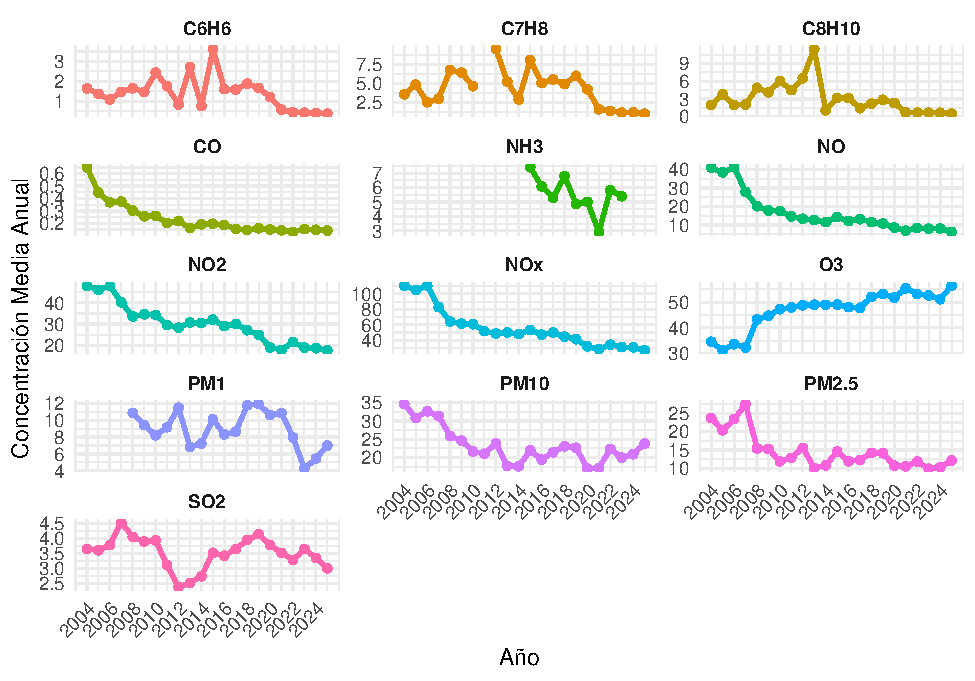
\includegraphics[width=0.75\linewidth]{ProyectoAED_Memoria_files/figure-latex/unnamed-chunk-9-1} 

}

\caption{Evolución de Variables Contaminantes (2004 - 2025)}\label{fig:unnamed-chunk-9}
\end{figure}

Vemos que la mayoría de sustancias cubren el periodo completo de 2004 a
2025, pero algunas (como \(PM_{1}\) y \(NH_3\)) solo tienen datos desde
2008 y 2015, respectivamente.

De forma similar, se analizaron las tendencias anuales de las variables
meteorológicas y ambientales clave, como la temperatura, la velocidad
del viento, la precipitación y el ruido. La Figura 2 presenta estos
resultados, de nuevo con escalas independientes para cada variable.

\begin{figure}[!h]

{\centering 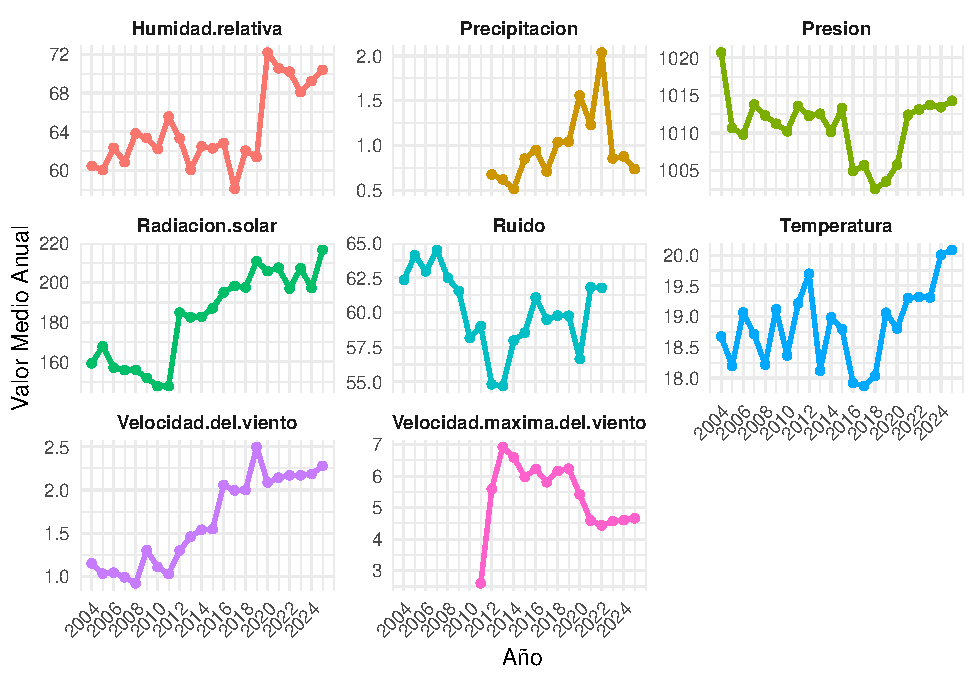
\includegraphics[width=0.75\linewidth]{ProyectoAED_Memoria_files/figure-latex/unnamed-chunk-10-1} 

}

\caption{Evolución de Variables Ambientales y Meteorológicas (2004 - 2025)}\label{fig:unnamed-chunk-10}
\end{figure}

Se observa que la variable de Precipitación y Velocidad máxima del
viento solo tienen valores desde 2011, mientras que la variable Ruido
solo tiene datos hasta 2022.

\subsection{Análisis de Cobertura y Disponibilidad de Datos por Estación
y
Año}\label{anuxe1lisis-de-cobertura-y-disponibilidad-de-datos-por-estaciuxf3n-y-auxf1o}

Además de analizar las tendencias de las medias anuales, es fundamental
evaluar la cobertura y disponibilidad de los datos. Un análisis del
número de registros por estación y año nos permite identificar qué
periodos y estaciones tienen datos suficientes para un análisis robusto.
La Figura 3 presenta esta distribución mediante un gráfico de barras
apiladas. El gráfico muestra un crecimiento en el volumen de registros
anuales, lo cual se debe a la expansión progresiva de la red de
vigilancia. Se observa cómo a las estaciones iniciales (como
\texttt{Viveros} y \texttt{Pista\ Silla}) se suman grandes
contribuyentes de datos a partir de 2010 y un nuevo grupo de estaciones
portuarias tras el 2020.

\begin{figure}[!h]

{\centering 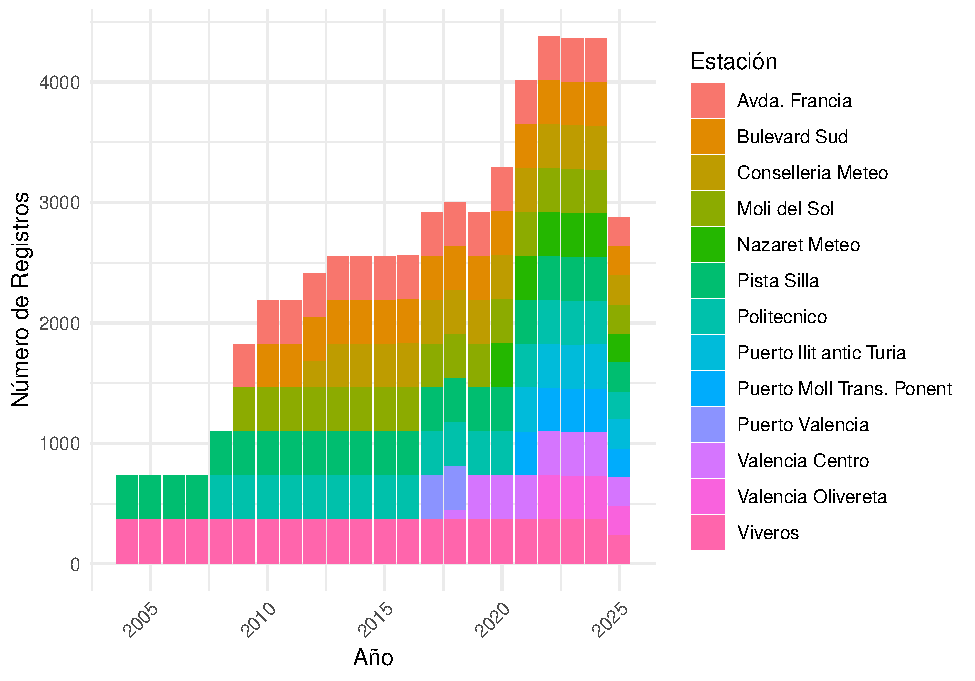
\includegraphics[width=0.6\linewidth]{ProyectoAED_Memoria_files/figure-latex/unnamed-chunk-11-1} 

}

\caption{Cobertura de Datos por Estación y Año.}\label{fig:unnamed-chunk-11}
\end{figure}

\section{Derivación de Variable Clave: Índice de Calidad del Aire
(ICA)}\label{derivaciuxf3n-de-variable-clave-uxedndice-de-calidad-del-aire-ica}

El Índice de Calidad del Aire (ICA) es una medida compuesta que
sintetiza la concentración de varios contaminantes en un solo valor,
facilitando la interpretación de la calidad del aire. En este capítulo,
se explica cómo se calcula el ICA a partir de las concentraciones
diarias de los contaminantes clave: \(PM_{10}\) (Partículas en
suspensión \(< 10 \mu m\)), \(PM_{2.5}\) (Partículas en suspensión
\(< 2.5 \mu m\)), \(NO_2\) (Dióxido de nitrógeno), \(O_3\) (Ozono) y
\(SO_2\) (Dióxido de azufre).

La definición utilizada (basada en el estándar europeo) establece que,
para reportar un índice de calidad del aire completo y representativo
del día para una ubicación es necesario tener la medición de todos los
contaminantes críticos para ese día en esa estación.

\subsection{Cálculo del ICA Diario por
Estación}\label{cuxe1lculo-del-ica-diario-por-estaciuxf3n}

Para el análisis, primero se cargaron los datos limpios. El paso clave
fue la creación de una función para calcular el Índice de Calidad del
Aire (ICA) Europeo.

Esta función asigna una categoría numérica (de 1 a 6) a la concentración
de cada contaminante según los umbrales establecidos por la normativa
europea. El ICA final del día es el valor máximo (el peor) de esos cinco
subíndices. Si falta un contaminante, no se puede saber si el subíndice
de ese contaminante faltante podría haber sido el peor de todos, lo que
llevaría a subestimar el riesgo real. La Figura 4 detalla los umbrales
de concentración (en \(\mu g/m^3\)) utilizados para cada contaminante y
categoría, que se corresponden con la lógica implementada en la función.

\begin{figure}[H]

{\centering 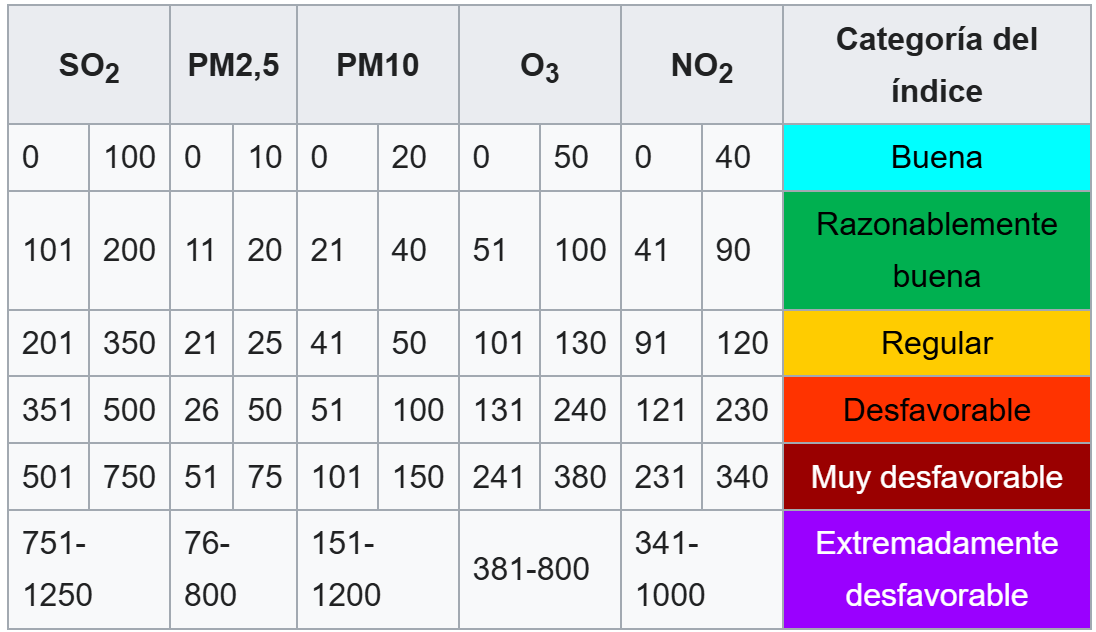
\includegraphics[width=0.6\linewidth]{ICA} 

}

\caption{Umbrales de Concentración para el Cálculo del Índice de Calidad del Aire (ICA) Europeo}\label{fig:umbrales_ica_imagen}
\end{figure}

\subsection{Exploración de Cobertura de Datos y Filtrado para el Cálculo
del
ICA}\label{exploraciuxf3n-de-cobertura-de-datos-y-filtrado-para-el-cuxe1lculo-del-ica}

El primer paso para derivar el ICA es una exploración de la cobertura.
Dado que el ICA requiere la medición simultánea de los cinco
contaminantes críticos, se calculó un ``ICA preliminar''. Este se marcó
como válido solo para los días y estaciones donde los cinco valores
estaban presentes. El objetivo era identificar qué estaciones de la red
miden, en algún momento, el conjunto completo de contaminantes.

\begin{verbatim}
## [1] "Estaciones válidas (miden los 5 contaminantes):"
\end{verbatim}

\begin{verbatim}
## [1] "Puerto Moll Trans. Ponent" "Puerto llit antic Turia"  
## [3] "Politecnico"               "Moli del Sol"             
## [5] "Avda. Francia"             "Pista Silla"              
## [7] "Viveros"
\end{verbatim}

Los resultados de la cobertura por estaciones muestran que solo 7 de las
12 estaciones tienen una cobertura superior al 0\%. Sin embargo, como se
observó en el análisis de cobertura anual (Figura 3), las estaciones del
Puerto son las más modernas y solo incluyen datos desde mediados de
2020, por lo que se decide eliminarlas del análisis del ICA para
mantener un conjunto de estaciones comparable a lo largo del tiempo,
quedando finalmente 5 estaciones válidas.

\begin{verbatim}
## Dataset filtrado a 34399 registros (5 estaciones).
\end{verbatim}

Tras el filtrado inicial de estaciones, se analizó la cobertura temporal
del ICA para las 5 estaciones restantes. El objetivo era identificar un
periodo de estudio coherente en el que todas las estaciones tuvieran
datos suficientes. La Figura 5 presenta esta la información en forma de
gráfico de calor, mostrando el porcentaje de cobertura de ICA para cada
estación-año. Los valores cercanos al 100\% (verde) indican una
cobertura completa, mientras que los valores bajos (rojo) señalan
periodos con datos insuficientes.

\begin{figure}[h!]

{\centering 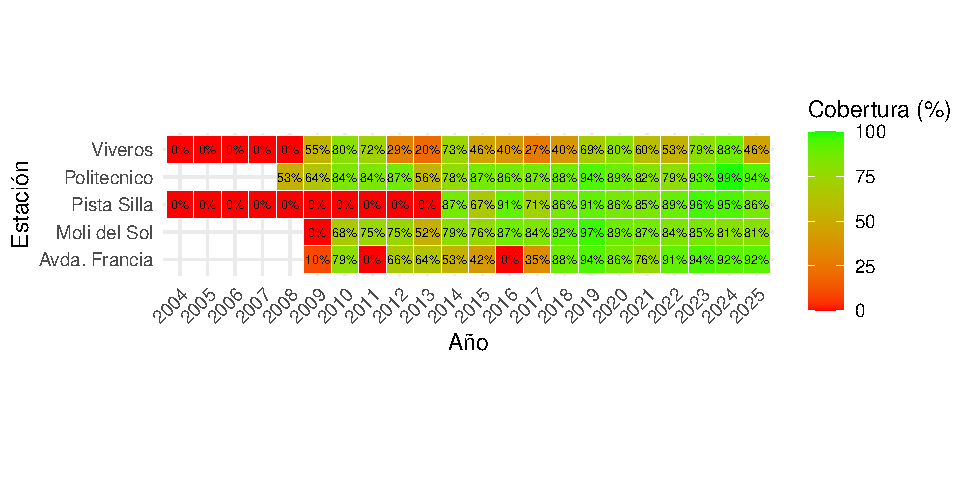
\includegraphics[width=1\linewidth]{ProyectoAED_Memoria_files/figure-latex/unnamed-chunk-16-1} 

}

\caption{Matriz de Cobertura Anual del ICA por Estación (2004-2025)}\label{fig:unnamed-chunk-16}
\end{figure}

Se observa que la cobertura antes de 2015 es incompleta y esporádica
para varias estaciones. Por lo tanto, para asegurar un análisis robusto
y comparable, se decidió filtrar de nuevo el dataset para incluir solo
los años con suficiente cobertura: enero de 2015 a agosto de 2025. Este
dataset filtrado de la última década será la base para el resto del
estudio.

\begin{verbatim}
## Dataset filtrado a 19424 registros (5 estaciones, 2015-2025).
\end{verbatim}

\subsection{Detección y Tratamiento de Outliers en Contaminantes
Críticos}\label{detecciuxf3n-y-tratamiento-de-outliers-en-contaminantes-cruxedticos}

Antes de calcular el ICA final, es crucial identificar y tratar los
valores atípicos (outliers) en las concentraciones de los contaminantes
críticos. Los outliers pueden distorsionar el cálculo del ICA y llevar a
interpretaciones erróneas de la calidad del aire. Para ello, se
generaron boxplots para cada contaminante crítico, permitiendo una
visualización clara de la distribución de los datos y la identificación
de posibles outliers.

\begin{center}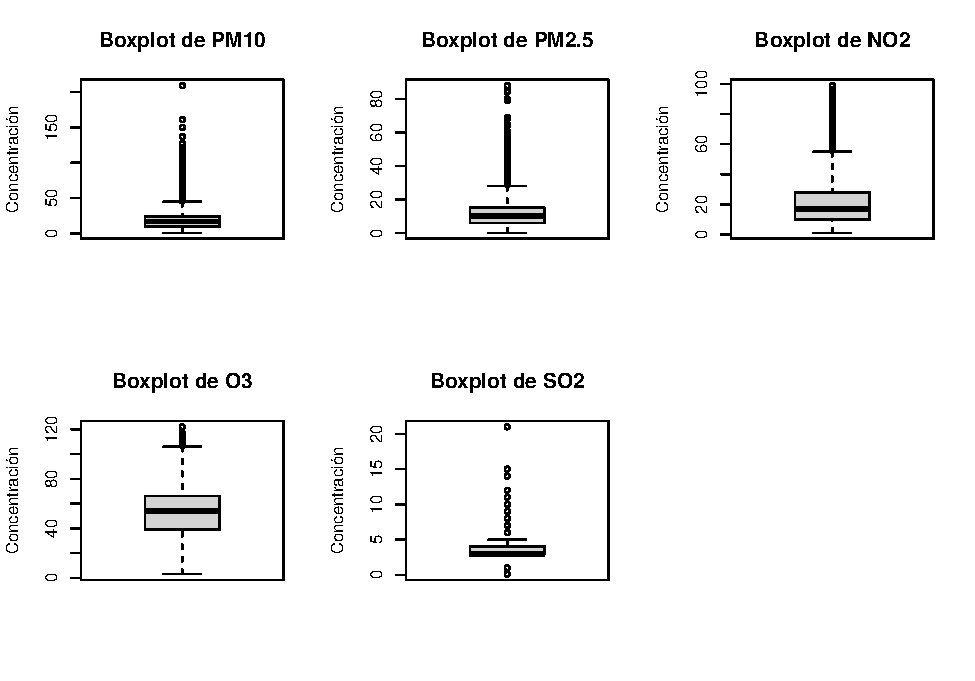
\includegraphics[width=0.75\linewidth]{ProyectoAED_Memoria_files/figure-latex/unnamed-chunk-18-1} \end{center}

Analizando los boxplots, se identificaron varios valores fuera de los
bigotes en las concentraciones de los contaminantes críticos. Sin
embargo, dado que estos valores atípicos por su magnitud podrían
representar episodios reales de contaminación, se decidió no eliminarlos
ni imputarlos en esta fase.

\subsection{Imputación de Valores
Faltantes}\label{imputaciuxf3n-de-valores-faltantes}

Dado que el cálculo del ICA requiere la presencia de todos los
contaminantes críticos, es necesario imputar los valores faltantes en el
dataset filtrado. Primero analizaremos qué cantidad de valores faltantes
hay en cada variable, y de qué tipo son.

\begin{figure}[!h]

{\centering 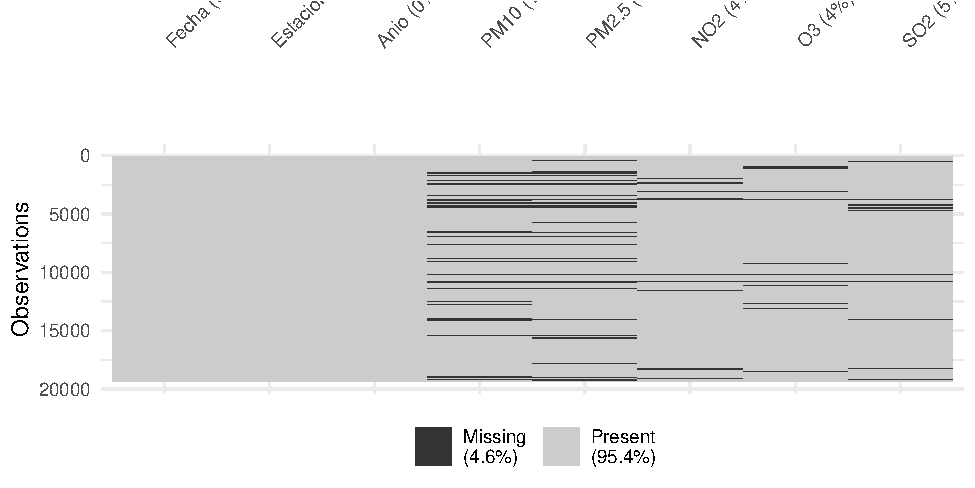
\includegraphics[width=0.65\linewidth]{ProyectoAED_Memoria_files/figure-latex/unnamed-chunk-19-1} 

}

\caption{Visualización de Valores Faltantes en Contaminantes Críticos (2015-2025)}\label{fig:unnamed-chunk-19}
\end{figure}

Observamos que, aunque hemos filtrado, todavía existen valores faltantes
dentro de nuestras 5 estaciones. Estos son los huecos que debemos
rellenar mediante imputación para tener una serie temporal completa.

En el gráfico observamos líneas negras horizontales como bloques de
filas, indicando que, para una observación específica, no falta solo una
variable faltan todas a la vez. Un fallo aleatorio no haría esto; esto
es un fallo sistemático, como por ejemplo que la estación entera se
apagó, estaba en mantenimiento, o se cortó la comunicación. Los datos
son probablemente MNAR, ya que los fallos en bloque no son eventos
aleatorios.

Por otro lado, también se ve que la mayoria de contaminantes tienen un
patrón de bloques faltantes diferente confirmando la hipótesis de que no
todas las estaciones miden siempre todas las variables del ICA. La falta
de ICA está perfectamente explicada por la falta de los contaminantes
que a su vez dependen de la variable Estación. Esto es lógico y es la
definición de MAR.

Para imputar los valores faltantes, utilizamos el método de
interpolación de Kalman (\texttt{na\_kalman} del paquete
\texttt{imputeTS}) basado en el filtro de Kalman, un algoritmo
estadístico que estima valores no observados en una serie temporal
aprovechando la información de los puntos anteriores y posteriores. Este
método permite reconstruir las series de cada estación de forma
coherente, continua y realista, sin introducir saltos artificiales ni
distorsionar la dinámica original de la serie temporal.

\subsection{Cálculo Final del ICA Diario por
Estación}\label{cuxe1lculo-final-del-ica-diario-por-estaciuxf3n}

Con los valores faltantes imputados, procedemos a calcular el ICA final
para cada estación y día en el periodo seleccionado (2015-2025). Podemos
observar la estructura final de este subdataset a continuación:

\begin{verbatim}
## Dataset ICA final guardado con 10 columnas y 19424 registros.
\end{verbatim}

\section{Creación del Dataset Analítico Agregado para el análisis de
correlación}\label{creaciuxf3n-del-dataset-analuxedtico-agregado-para-el-anuxe1lisis-de-correlaciuxf3n}

En este capítulo, explicamos cómo se construyó el dataset analítico
agregado que se utilizará para el análisis de correlación entre el ICA y
las variables meteorológicas y de fuentes de contaminación. Este
subdataset es esencial para analizar relaciones entre el ICA y el resto
de variables del conjunto de datos.

\subsection{Exploración de Cobertura de Datos y Filtrado para las
Variables
Explicativas}\label{exploraciuxf3n-de-cobertura-de-datos-y-filtrado-para-las-variables-explicativas}

Para analizar la correlación entre el ICA y factores externos, fue
necesario construir un dataset analítico agregado. El desafío es que las
variables explicativas (como la meteorología o indicadores de tráfico)
no se miden necesariamente en las mismas 5 estaciones donde se calculó
el ICA. Por lo tanto, el objetivo fue seleccionar la estación fuente más
fiable para cada variable explicativa y usarla como representante de la
ciudad. Para tomar esta decisión, se analizó la cobertura de datos para
cada variable en cada estación durante el periodo de estudio
(2015-2025).

\begin{figure}[!h]

{\centering 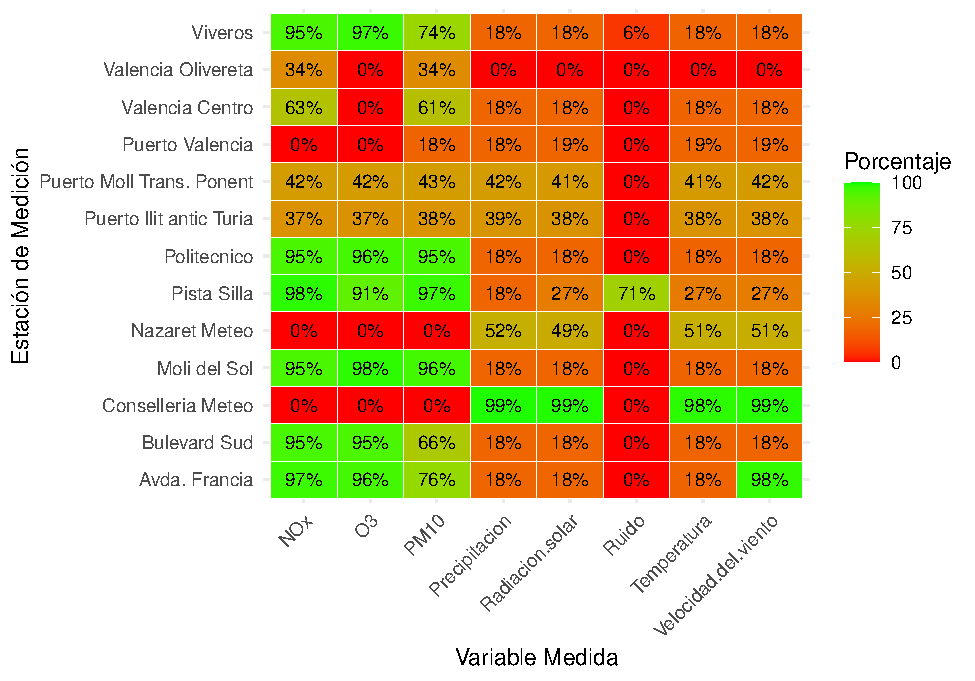
\includegraphics[width=0.75\linewidth]{ProyectoAED_Memoria_files/figure-latex/unnamed-chunk-23-1} 

}

\caption{Matriz de Cobertura de Variables Explicativas por Estación}\label{fig:unnamed-chunk-23}
\end{figure}

De el \texttt{heatmap} se observa que para las variables de
meteorología, la estación Conselleria Meteo tiene una cobertura
\textgreater98\% para todas las variables meteorológicas, por lo que es
la fuente idónea. Para el tráfico, la estación Pista Silla ofrece la
mejor cobertura para los contaminantes considerados \(NO_x\) y
\(PM_{10}\). Para el Ozono el Politecnico es la fuente más completa
(96\%). Y por último, se observa que la cobertura de Ruido es del 71\%
en `Pista Silla', pero como se vio en el análisis de tendencias (Figura
2), el registro se interrumpe en 2022. Por tanto, se excluye esta
variable del análisis de correlación final.Basado en esto, se extrajeron
las series temporales de estas estaciones fuente, se promedió el ICA de
las 5 estaciones para obtener un valor diario de la ciudad, y se unió
todo en un único dataset analítico ``ancho'', con una fila por día y
todas las variables explicativas junto al ICA diario promedio.

\begin{verbatim}
## Dataset analítico creado con 3896 registros y 9 variables.
\end{verbatim}

\subsection{Detección y Tratamiento de Outliers en el Dataset
Analítico}\label{detecciuxf3n-y-tratamiento-de-outliers-en-el-dataset-analuxedtico}

De la misma manera que antes, exploramos los posibles valores atípicos
en el dataset analítico resultante para decidir cómo tratarlos.

\begin{figure}[!h]

{\centering 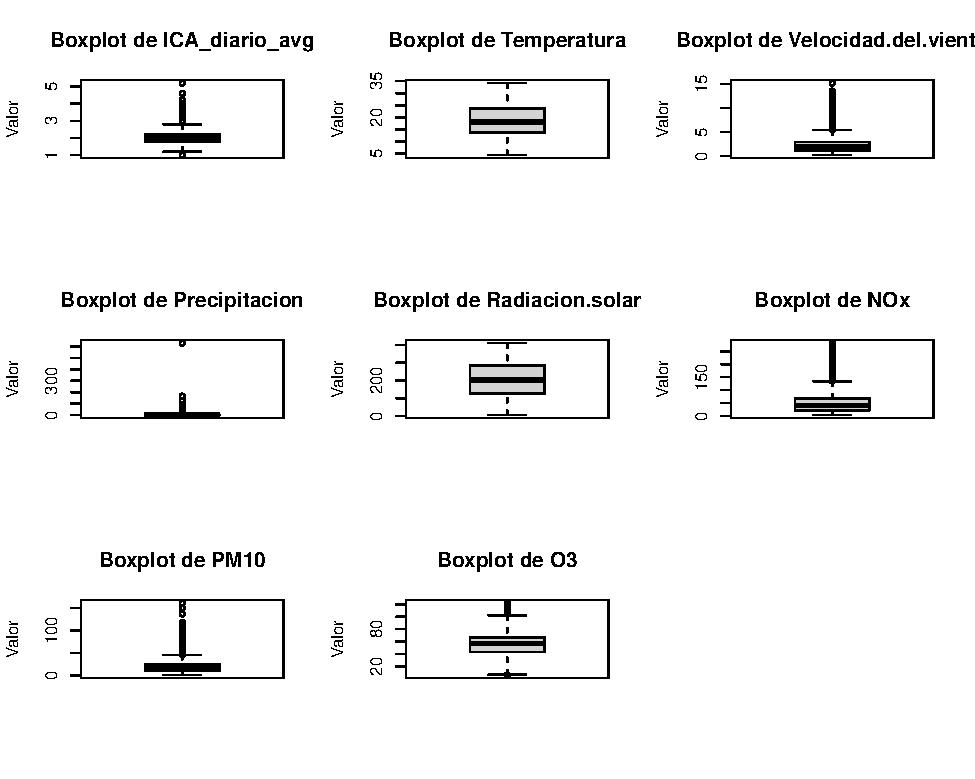
\includegraphics[width=0.7\linewidth]{ProyectoAED_Memoria_files/figure-latex/unnamed-chunk-27-1} 

}

\caption{Boxplots de Variables Explicativas en el Dataset Analítico}\label{fig:unnamed-chunk-27}
\end{figure}

De nuevo, observamos que los valores atípicos no son de magnitud
imposible para las variables, simplemente podrían tratarse de días de
más o menos contaminación o condiciones meteorológicas extremas, por lo
que los dejaremos tal y como están.

Salvo un valor de precipitación extremadamente alto (más de 600 mm en un
día), que parece un error de registro, por lo que lo sustituiremos por
\texttt{NA} para que sea imputado posteriormente.

Podríamos pensar que ese valor fue durante la DANA el 29 de octubre de
2024, sin embargo, si lo localizamos en el dataset vemos que no
corresponde a esa fecha, sino al 27 de septiembre de 2022, por lo que
parece un error de registro, Así que lo sustituimos por \texttt{NA}.

\subsection{Imputación Final de Valores Faltantes en las Variables
Explicativas}\label{imputaciuxf3n-final-de-valores-faltantes-en-las-variables-explicativas}

Analizamos los valores faltantes en las variables explicativas
seleccionadas.

\begin{figure}[!h]

{\centering 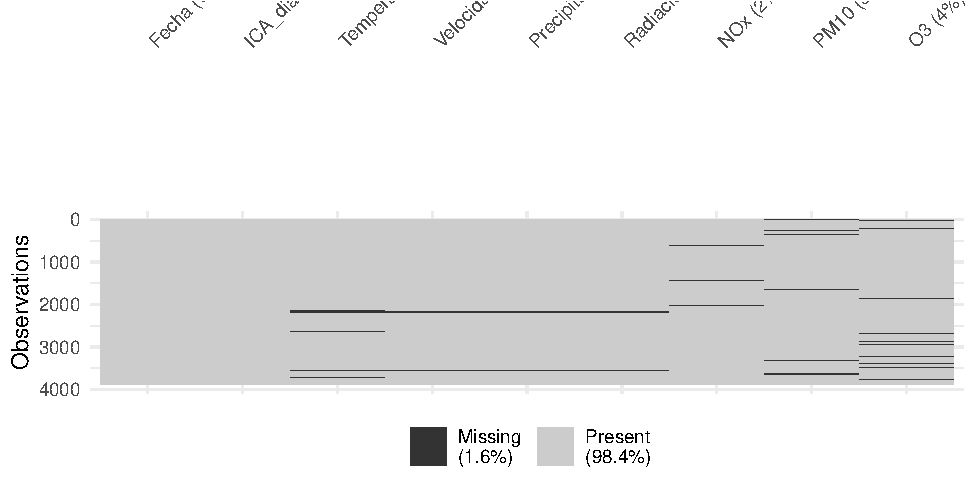
\includegraphics[width=0.6\linewidth]{ProyectoAED_Memoria_files/figure-latex/unnamed-chunk-30-1} 

}

\caption{Visualización de Valores Faltantes en el Dataset Analítico}\label{fig:unnamed-chunk-30}
\end{figure}

En el gráfico, los datos mostrados presentan un patrón de ausencia no
aleatoria: los huecos aparecen en bloques horizontales que afectan
simultáneamente a varias variables, sobre todo entre variables
meteorológicas o de tráfico, por separado. Esto indica un fallo
sistemático como por ejemplo, la interrupción del registro en una
estación o mantenimiento del sensor. Por tanto, los valores faltantes
pueden explicarse por variables observadas (como la estación o la falta
simultánea en otros contaminantes), se clasifican como MAR.

Aplicamos la imputación de Kalman a todas las variables explicativas en
el dataset analítico.

Finalmente, guardamos el dataset analítico completo y listo para el
análisis entre variables posterior.

\begin{verbatim}
## Dataset analítico final guardado con 3896 registros.
\end{verbatim}

\section{Resultados}\label{resultados}

Los pasos anteriores de preparación yde datos nos han permitido crear
dos datasets limpios y completos que emplearemos para responder a los
análisis planteados en la introducción. En este capítulo, presentamos
los resultados obtenidos a partir del análisis descriptivo del ICA y su
correlación con las variables explicativas seleccionadas.

\subsection{Análisis Descriptivo del ICA por
Estación}\label{anuxe1lisis-descriptivo-del-ica-por-estaciuxf3n}

El primer análisis se centra en describir la distribución y patrones del
Índice de Calidad del Aire (ICA) en las estaciones seleccionadas durante
el periodo 2015-2025.

\subsubsection{Análisis univariante del
ICA}\label{anuxe1lisis-univariante-del-ica}

Graficamos la distribución general del ICA, con tal de determinar que
días son más frecuentes, si los de buena, moderada o mala calidad.

\begin{figure}[!h]

{\centering 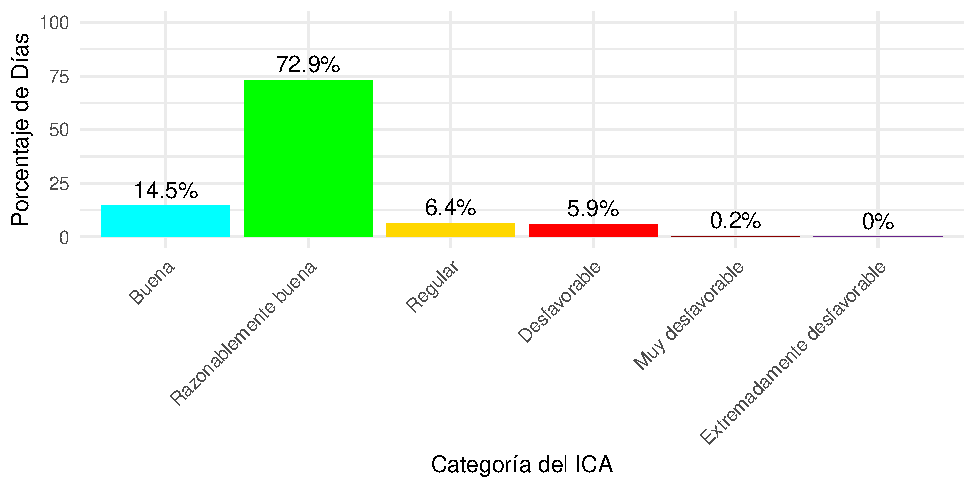
\includegraphics[width=0.75\linewidth]{ProyectoAED_Memoria_files/figure-latex/unnamed-chunk-34-1} 

}

\caption{Distribución del Índice de Calidad del Aire (ICA) por Categoría (2015-2025)}\label{fig:unnamed-chunk-34}
\end{figure}

Como era de esperar, del gráfico de barras se observa que la mayoría de
los días tienen una calidad del aire buena o razonablemente buena, con
un porcentaje mucho más bajo de días con calidad regular o desfavorable.
De hecho, la última categoría de ``Extremadamente desfavorable'' no
cuenta con ningún registro. Esto indica que, en general, la calidad
general del aire en Valencia, según los datos de las 5 estaciones
consideradas entre 2015 y 2025, es predominantemente buena.

\subsubsection{Análisis bivariante del
ICA}\label{anuxe1lisis-bivariante-del-ica}

En un segundo análisis, exploramos los patrones temporales y espaciales
del ICA para identificar tendencias y variaciones significativas a lo
largo del tiempo y entre las estaciones.

\paragraph{\texorpdfstring{\textbf{Análisis
Temporal}}{Análisis Temporal}}\label{anuxe1lisis-temporal}

Primero, analizamos cómo ha evolucionado el ICA a lo largo del tiempo,
identificando tendencias generales y patrones específicos durante
eventos relevantes como el confinamiento por la pandemia de COVID-19.

\begin{figure}[!h]

{\centering 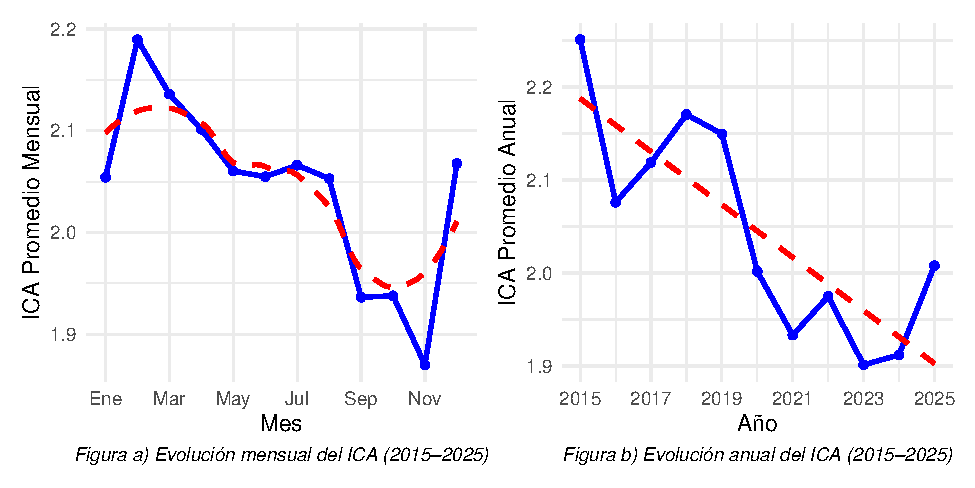
\includegraphics[width=0.8\linewidth]{ProyectoAED_Memoria_files/figure-latex/unnamed-chunk-36-1} 

}

\caption{Evolución Temporal del Índice de Calidad del Aire (ICA) Promedio Mensual y Anual (2015-2025)}\label{fig:unnamed-chunk-36}
\end{figure}

Analizando el gráfico de líneas del ICA promedio mensual, podemos
observar un patrón estacional claro en la calidad del aire en Valencia.
Los meses de invierno (diciembre a febrero) tienden a mostrar valores
más altos de ICA, indicando una peor calidad del aire, posiblemente
debido a factores como la inversión térmica y el aumento de las
emisiones por calefacción. En contraste, los meses de verano (junio a
agosto) presentan los valores más bajos de ICA, reflejando una mejor
calidad del aire, probablemente influenciada por condiciones
meteorológicas favorables y una menor actividad industrial y de
vehículos en la ciudad.

Como se observa, el ICA promedio anual muestra una tendencia general que
disminuye a lo largo del periodo 2015-2025, indicando una pequeña mejora
la calidad del aire en Valencia. El eje Y varía de aproximadamente 2.25
a 2.0 en los últimos años indicando una mejora gradual aunque muy leve
en la calidad del aire. Realmente dado que estamos en 2025 y nuestros
registros únicamente son hasta agosto, el valor promedio anual que
aumenta con respecto a 2024 no es fiable todavía, poríamos analizarlo al
contar con los registros hasta final de año.

En cuanto al periodo del confinamiento por la pandemia de COVID-19
(marzo-junio 2020), podríamos sostener la hipótesis de que hubo una
caída drástica en el ICA debido a la reducción significativa de las
actividades humanas y el tráfico durante ese tiempo.

\begin{figure}[!h]

{\centering 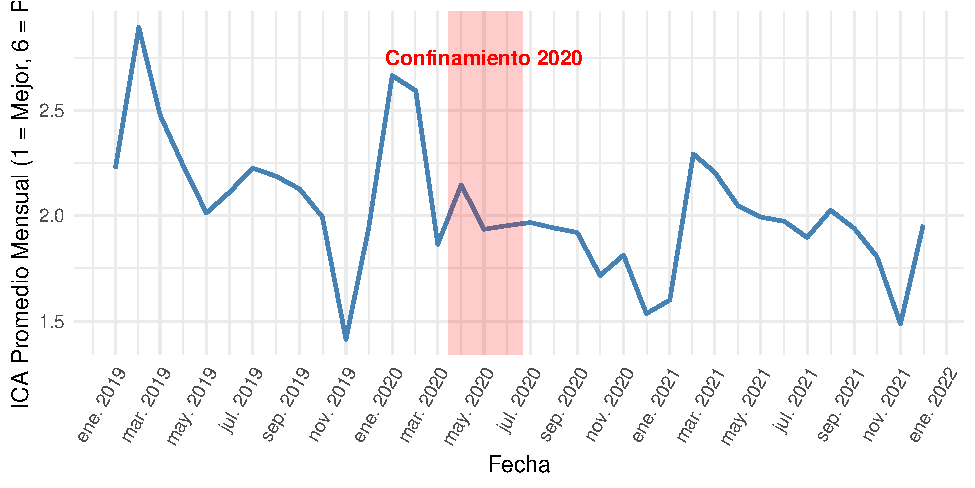
\includegraphics[width=0.65\linewidth]{ProyectoAED_Memoria_files/figure-latex/unnamed-chunk-37-1} 

}

\caption{Evolución Temporal del Índice de Calidad del Aire (ICA) Promedio Mensual con Resalte del Confinamiento por COVID-19 (2019-2021)}\label{fig:unnamed-chunk-37}
\end{figure}

Si observamos el gráfico, justo el mes antes del antes del
confinamiento, el ICA promedio mensual era de aproximadamente 2.5. Sin
embargo, justo antes de entrar en el confinamiento en marzo de 2020, el
ICA cae a alrededor de 2.0. Durante el periodo de confinamiento (marzo a
junio de 2020), el ICA se mantiene bajo, alrededor de 1.9, pudiendo
deberse a la reducción del tráfico y las actividades industriales,
podría ser un punto a estudiar. Si lo comparamos con los mismos meses
del año anterior, los valores estaban alrededor de 2.2, un poco más
altos. A principios del 2021, el ICA vuelve a aumentar nuevamente hasta
2.3 aprox.

\paragraph{\texorpdfstring{\textbf{Análisis
espacial}}{Análisis espacial}}\label{anuxe1lisis-espacial}

En este apartado, analizamos cómo varía el ICA entre las diferentes
estaciones de medición para identificar áreas con peor calidad del aire
o si la calidad es uniforme en toda la ciudad.

\begin{figure}[!h]

{\centering 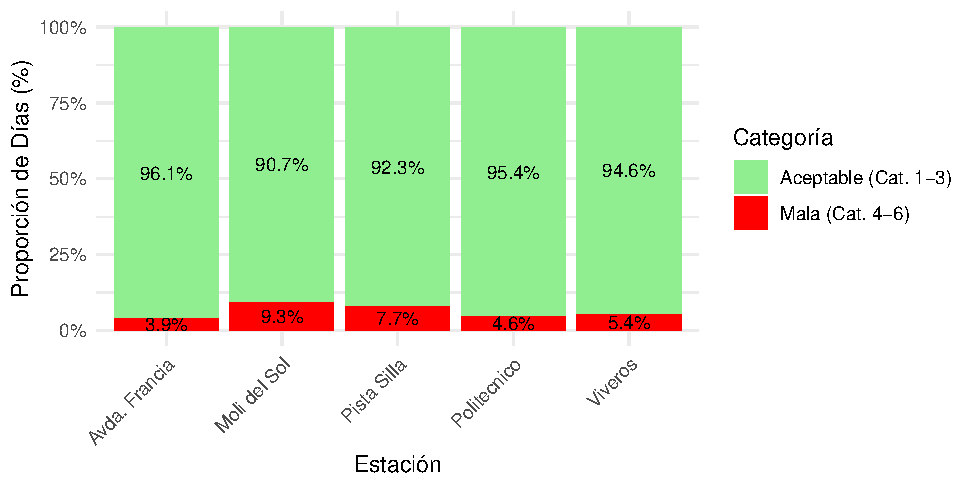
\includegraphics[width=0.75\linewidth]{ProyectoAED_Memoria_files/figure-latex/unnamed-chunk-38-1} 

}

\caption{Proporción de Días con Calidad del Aire 'Mala' vs 'Aceptable' por Estación (2015-2025)}\label{fig:unnamed-chunk-38}
\end{figure}

Analizando el gráfico de barras apiladas, podemos observar que aen todas
las estaciones la mayoría de registros son de buena calidad.La estación
con peor calidad del aire es Moli del Sol con casi el 10\% de registros
de mala calidad, seguida de la ubicada en la Pista de Silla con un
aprox. 8\%. Estas dos estaciones se localizan en zonas con alta densidad
de tráfico rodado y actividad industrial, lo que explica la mayor
concentración de contaminantes primarios y, por tanto, un ICA más
elevado.

Por último, analizamos las diferencias en la calidad entre los días
laborables y los fines de semana.

\begin{figure}[!h]

{\centering 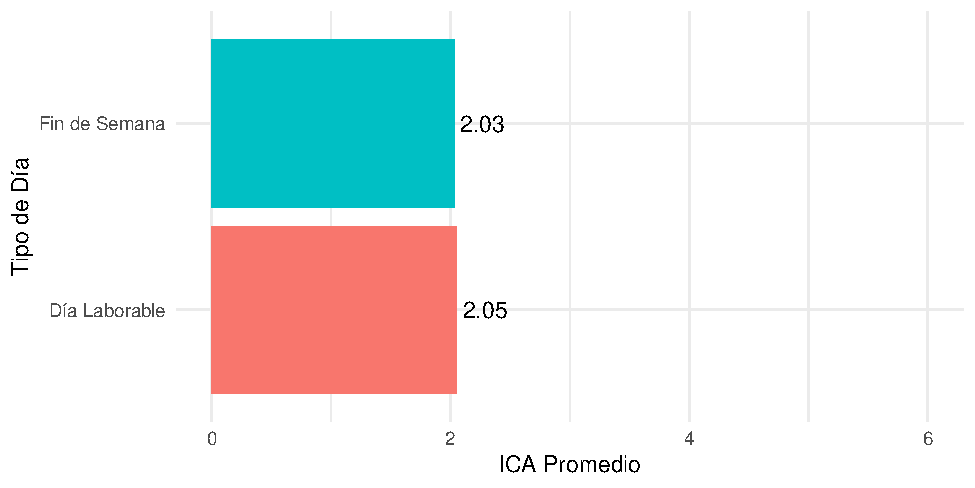
\includegraphics[width=0.65\linewidth]{ProyectoAED_Memoria_files/figure-latex/unnamed-chunk-39-1} 

}

\caption{Comparación del Índice de Calidad del Aire (ICA) Promedio: Días Laborables vs Fines de Semana (2015-2025)}\label{fig:unnamed-chunk-39}
\end{figure}

No hay una diferencia significativa en el ICA promedio entre días
laborables y fines de semana. Ambos tipos de días presentan un ICA
promedio similar. .Sin embargo, es posible que haya diferencias en los
niveles de contaminantes específicos debido a variaciones en las
actividades humanas y el tráfico durante estos días.

Por lo que podemos comparar 2 de los contaminantes principales del ICA,
el \(NO_2\) y el \(O_3\), entre días laborables y fines de semana.

\begin{figure}[!h]

{\centering 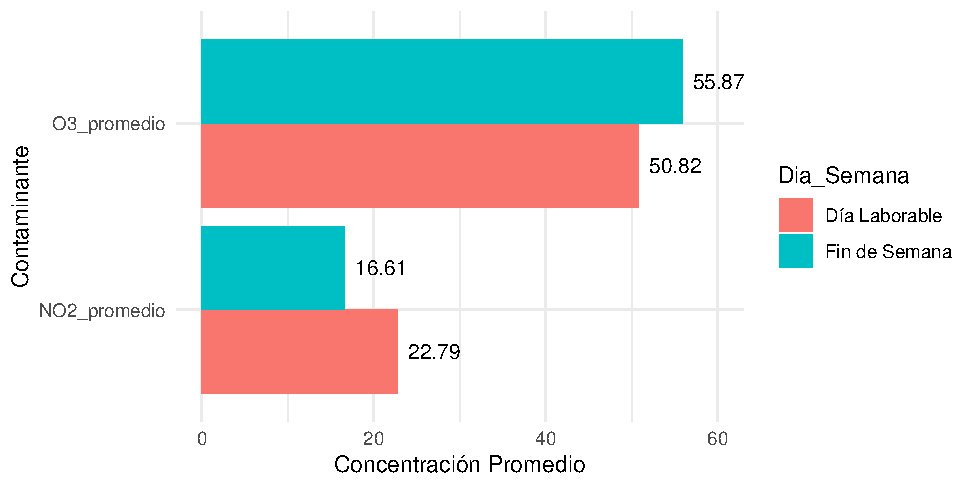
\includegraphics[width=0.75\linewidth]{ProyectoAED_Memoria_files/figure-latex/unnamed-chunk-40-1} 

}

\caption{Comparación de Concentraciones Promedio de NO2 y O3: Días Laborables vs Fines de Semana (2015-2025)}\label{fig:unnamed-chunk-40}
\end{figure}

El gráfico de barras muestra que el \(NO_2\) tiene una concentración
promedio más alta en días laborables en comparación con los fines de
semana, lo cual es consistente con la mayor actividad vehicular durante
los días laborables. Por otro lado, el \(O_3\) presenta una
concentración promedio ligeramente más alta durante los fines de semana,
lo que podría tiene sentido ya que las emisiones de NO se reducen, lo
que reduce la destrucción del ozono troposférico. En consecuencia, las
concentraciones medias de \(O_3\) suelen ser ligeramente más elevadas, a
pesar de que las emisiones totales de contaminantes primarios son
menores.

\subsection{Análisis de Correlación del ICA con las Variables
Explicativas}\label{anuxe1lisis-de-correlaciuxf3n-del-ica-con-las-variables-explicativas}

En este capítulo, exploramos las relaciones entre el ICA y las variables
meteorológicas y de fuentes de contaminación seleccionadas en el dataset
analítico. El objetivo es identificar qué factores influyen más
significativamente en la calidad del aire en Valencia.

\subsubsection{Influencia de la
Meteorología}\label{influencia-de-la-meteorologuxeda}

Por un lado, podemos analizar la correlación entre el ICA y las
diferentes variables meteorológicas seleccionadas: Temperatura,
Velocidad del Viento, Precipitación y Radiación Solar.

\begin{figure}[!h]

{\centering 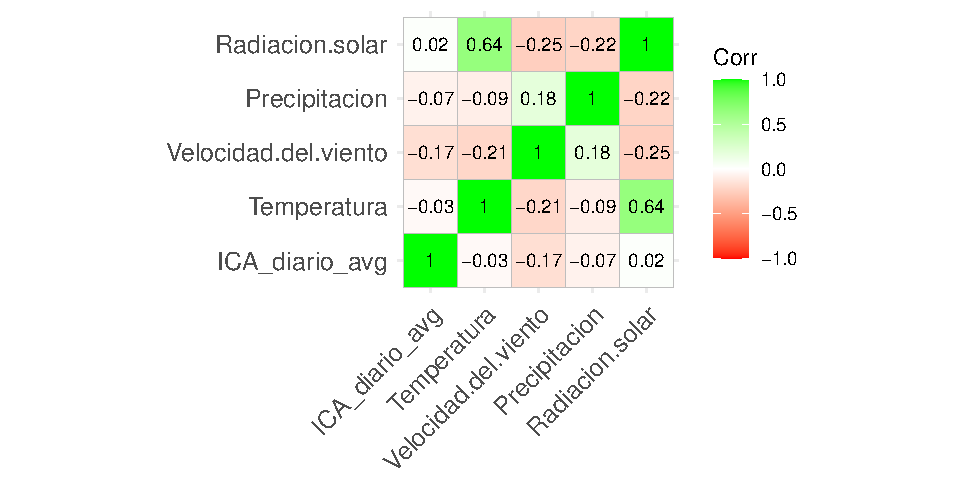
\includegraphics[width=0.75\linewidth]{ProyectoAED_Memoria_files/figure-latex/unnamed-chunk-41-1} 

}

\caption{Matriz de Correlación entre el Índice de Calidad del Aire (ICA) y Variables Meteorológicas (2015-2025)}\label{fig:unnamed-chunk-41}
\end{figure}

Analizando la matriz de correlación, podemos observar que en general,
las correlaciones son débiles, lo que sugiere que la calidad del aire
resulta de la interacción de varios factores simultáneos. Resulta
evidente la alta correlación entre la temperatura y la radiación solar.

Como punto extra a analizar, podemos explorar como la temperatura y la
radiación solar influyen en los niveles de ozono (\(O_3\)), un
contaminante secundario que se forma por reacciones fotoquímicas a
partir de \(NO_2\) en presencia de luz.

\begin{figure}[!h]

{\centering 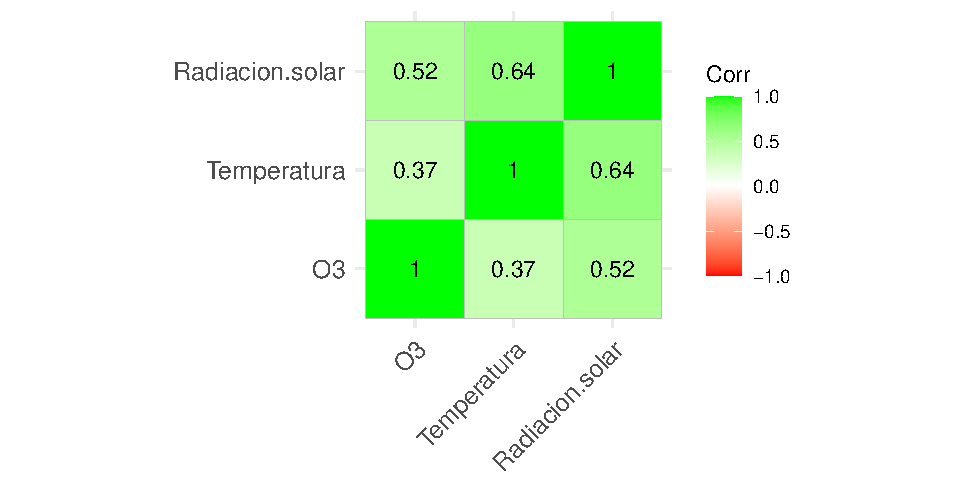
\includegraphics[width=0.75\linewidth]{ProyectoAED_Memoria_files/figure-latex/unnamed-chunk-42-1} 

}

\caption{Matriz de Correlación entre Ozono (O3), Temperatura y Radiación Solar (2015-2025)}\label{fig:unnamed-chunk-42}
\end{figure}

Como se observa en la matriz de correlación, el ozono (\(O_3\)) muestra
una correlación positiva moderada con la radiación solar (0.57) y una
correlación más débil con la temperatura pero también positiva (0.37).
Esto indica que a medida que aumentan la temperatura y la radiación
solar, los niveles de ozono tienden a incrementarse, lo cual es
consistente con el conocimiento científico sobre la formación de ozono
troposférico a través de reacciones fotoquímicas.

\subsubsection{Influencia de Fuentes de
Contaminación}\label{influencia-de-fuentes-de-contaminaciuxf3n}

Por último, analizamos la correlación entre el ICA y las variables
relacionadas con fuentes de contaminación, específicamente \(NO_x\) y
\(PM_{10}\). El \(NO_x\) es un contaminante primario emitido
principalmente por el tráfico vehicular, mientras que el \(PM_{10}\)
puede tener múltiples fuentes, incluyendo emisiones industriales y polvo
en suspensión.

\begin{figure}[!h]

{\centering 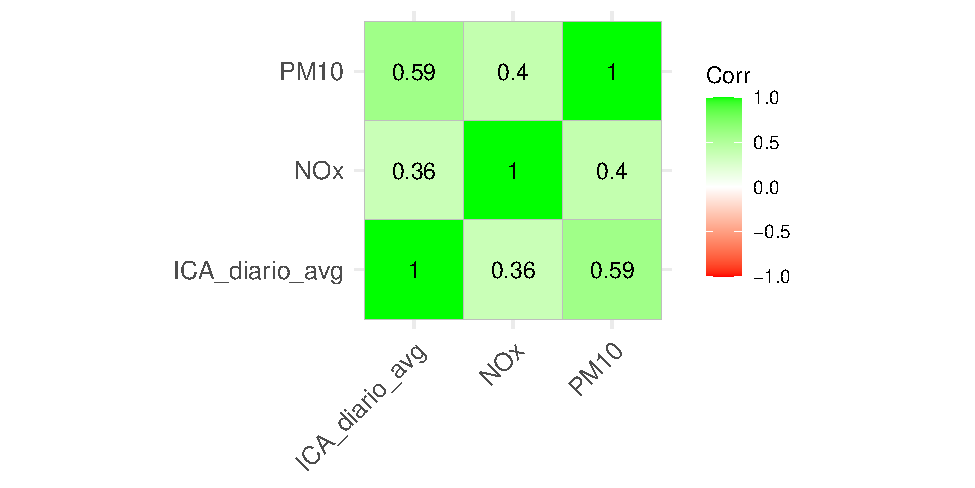
\includegraphics[width=0.75\linewidth]{ProyectoAED_Memoria_files/figure-latex/unnamed-chunk-43-1} 

}

\caption{Matriz de Correlación entre el Índice de Calidad del Aire (ICA) y Contaminantes Primarios (2015-2025)}\label{fig:unnamed-chunk-43}
\end{figure}

Analizando la matriz de correlación, podemos observar que tanto el
\(NO_x\) como el \(PM_{10}\) muestran una correlación positiva moderada
con el ICA. Esto confirma parcialmente lo que se conoce como ``huella de
tráfico'' indicando que a medida que aumentan las concentraciones de
estos contaminantes primarios, la calidad del aire empeora (ICA más
alto). Concretamente la variable de partículas suspendidas de hasta
\(10\mu m\) tiene una correlación de un 0.59, lo cual es lógico ya que
es una de las sustancias principales para el cálculo del índice. Como
último análisis, se podría considerar la variación de estas sustancias a
lo largo del tiempo para analizar sus tendencias y patrones
estacionales, y así confirmar si su comportamiento temporal coincide con
el de la actividad humana.

\begin{figure}[!h]

{\centering 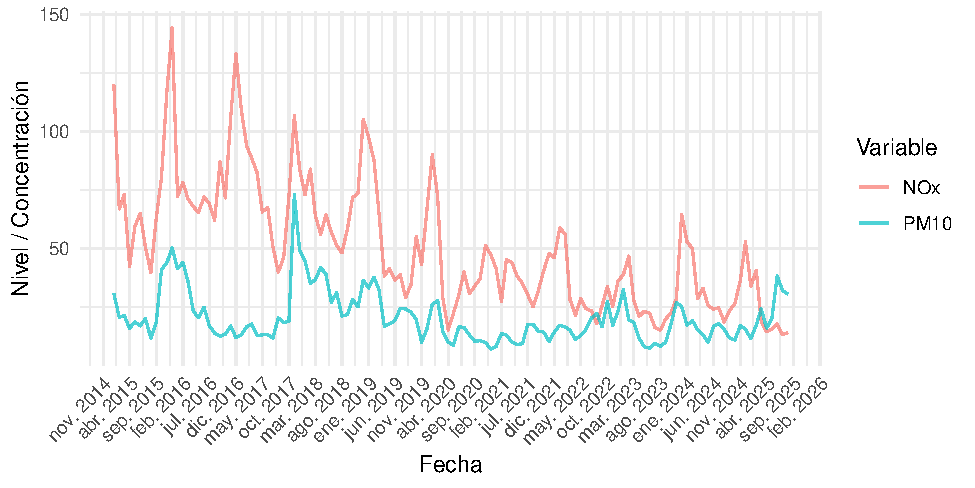
\includegraphics[width=0.75\linewidth]{ProyectoAED_Memoria_files/figure-latex/unnamed-chunk-44-1} 

}

\caption{Evolución Temporal de NOx y PM10 (2015-2025)}\label{fig:unnamed-chunk-44}
\end{figure}

En la gráfica de líneas, podemos observar que tanto el \(NO_x\) como el
\(PM_{10}\) presentan patrones estacionales similares, con picos más
altos durante los meses de invierno y valores más bajos en verano. Esto
puede estar relacionado con factores meteorológicos como la temperatura
y la estabilidad atmosférica, que afectan la dispersión de los
contaminantes.

Además, se observa una tendencia general a la baja sobre todo en el
\(NO_x\) a lo largo del periodo 2015-2025, lo que podría indicar mejoras
en las políticas de control de emisiones y la calidad del aire en
Valencia.

\section{Conclusiones}\label{conclusiones}

Este proyecto ha consistido en un completo proceso de Análisis
Exploratorio de Datos. En primer lugar, se abordó la tarea fundamental
de fusionar y consolidar múltiples conjuntos de datos sobre la calidad
del aire (2004-2025) provenientes de fuentes distintas (Ayuntamiento de
Valencia y GVA), que presentaban formatos y estructuras muy diferentes.
El núcleo del trabajo se centró en una fase de preparación y limpieza,
indispensable para asegurar la fiabilidad del análisis. Esto incluyó la
estandarización de variables y un análisis de los valores atípicos
(outliers) para evaluar la coherencia de las mediciones.

Además, para la gestión de los valores faltantes, se optó por aplicar
técnicas de imputación estadística para rellenar los huecos de manera
robusta. Esto permitió construir una serie temporal completa y robusta
para el periodo de estudio principal (2015-2025). Con esta base de datos
sólida, se derivó la variable clave del Índice de Calidad del Aire (ICA)
y se aplicaron distintas técnicas analíticas: desde el análisis
univariante (para entender la distribución de la calidad del aire) y
bivariante (para comparar patrones entre estaciones o épocas del año),
hasta el análisis de correlaciones (para identificar relaciones entre la
contaminación y factores como el tráfico o la meteorología). El uso de
múltiples visualizaciones gráficas fue esencial en cada etapa para
detectar patrones y tomar decisiones durante el proceso de exploración.

%%%%%%%%%%%%%%%%%%%%%%%%%%%%%%%%%%%%%%%%%%

\vspace{6pt}

%%%%%%%%%%%%%%%%%%%%%%%%%%%%%%%%%%%%%%%%%%
%% optional

% Only for the journal Methods and Protocols:
% If you wish to submit a video article, please do so with any other supplementary material.
% \supplementary{The following supporting information can be downloaded at: \linksupplementary{s1}, Figure S1: title; Table S1: title; Video S1: title. A supporting video article is available at doi: link.}

% Only for journal Hardware:
% If you wish to submit a video article, please do so with any other supplementary material.
% \supplementary{The following supporting information can be downloaded at: \linksupplementary{s1}, Figure S1: title; Table S1: title; Video S1: title.\vspace{6pt}\\
%\begin{tabularx}{\textwidth}{lll}
%\toprule
%\textbf{Name} & \textbf{Type} & \textbf{Description} \\
%\midrule
%S1 & Python script (.py) & Script of python source code used in XX \\
%S2 & Text (.txt) & Script of modelling code used to make Figure X \\
%S3 & Text (.txt) & Raw data from experiment X \\
%S4 & Video (.mp4) & Video demonstrating the hardware in use \\
%... & ... & ... \\
%\bottomrule
%\end{tabularx}
%}

%%%%%%%%%%%%%%%%%%%%%%%%%%%%%%%%%%%%%%%%%%




\dataavailability{Los datos presentados en este estudio son de dominio
público y están disponibles

abiertamente en sus fuentes originales: Portal de Datos Abiertos del
Ayuntamiento de Valencia
(\url{https://valencia.opendatasoft.com/pages/home/})) y Portal de
Calidad Ambiental de la Generalitat Valenciana
(\url{https://mediambient.gva.es/es/web/calidad-ambiental/calidad-del-aire})}

% Only for journal Nursing Reports
%\publicinvolvement{Please describe how the public (patients, consumers, carers) were involved in the research. Consider reporting against the GRIPP2 (Guidance for Reporting Involvement of Patients and the Public) checklist. If the public were not involved in any aspect of the research add: ``No public involvement in any aspect of this research''.}

% Only for journal Nursing Reports
%\guidelinesstandards{Please add a statement indicating which reporting guideline was used when drafting the report. For example, ``This manuscript was drafted against the XXX (the full name of reporting guidelines and citation) for XXX (type of research) research''. A complete list of reporting guidelines can be accessed via the equator network: \url{https://www.equator-network.org/}.}

% Only for journal Nursing Reports
%\guidelinesstandards{Please add a statement indicating which reporting guideline was used when drafting the report. For example, ``This manuscript was drafted against the XXX (the full name of reporting guidelines and citation) for XXX (type of research) research''. A complete list of reporting guidelines can be accessed via the equator network: \url{https://www.equator-network.org/}.}



%%%%%%%%%%%%%%%%%%%%%%%%%%%%%%%%%%%%%%%%%%
%% Optional

%% Only for journal Encyclopedia
%\entrylink{The Link to this entry published on the encyclopedia platform.}


%%%%%%%%%%%%%%%%%%%%%%%%%%%%%%%%%%%%%%%%%%
%% Optional
%%%%%%%%%%%%%%%%%%%%%%%%%%%%%%%%%%%%%%%%%%
\begin{adjustwidth}{-\extralength}{0cm}

%\printendnotes[custom] % Un-comment to print a list of endnotes



% If authors have biography, please use the format below
%\section*{Short Biography of Authors}
%\bio
%{\raisebox{-0.35cm}{\includegraphics[width=3.5cm,height=5.3cm,clip,keepaspectratio]{Definitions/author1.pdf}}}
%{\textbf{Firstname Lastname} Biography of first author}
%
%\bio
%{\raisebox{-0.35cm}{\includegraphics[width=3.5cm,height=5.3cm,clip,keepaspectratio]{Definitions/author2.jpg}}}
%{\textbf{Firstname Lastname} Biography of second author}

%%%%%%%%%%%%%%%%%%%%%%%%%%%%%%%%%%%%%%%%%%
%% for journal Sci
%\reviewreports{\\
%Reviewer 1 comments and authors’ response\\
%Reviewer 2 comments and authors’ response\\
%Reviewer 3 comments and authors’ response
%}
%%%%%%%%%%%%%%%%%%%%%%%%%%%%%%%%%%%%%%%%%%
\PublishersNote{}
\end{adjustwidth}


\end{document}
